\documentclass[journal, table]{IEEEtran}
\usepackage[english, spanish]{babel}
\usepackage[sorting=none]{biblatex}
\bibliography{ref.bib}
\usepackage{amsmath, amsfonts, amsthm}
\usepackage{hyperref, url}
\hyphenation{op-tical net-works semi-conduc-tor}
\usepackage{graphicx}
\usepackage{float}
\usepackage{fancyhdr, last page}
\usepackage{siunitx}
\usepackage{anyfontsize}
\usepackage{csquotes}
\usepackage{svg}
\usepackage{tabularx, ragged2e, booktabs}
\usepackage{xcolor}
\usepackage{multirow}
\usepackage{adjustbox}
\usepackage[affil-sl]{authblk}
\usepackage[electronic]{ifsym}
\usepackage{tikz}
\usepackage[spanish]{cleveref}
\usepackage{circuitikz}
\usetikzlibrary{patterns}
\usepackage{scalerel}
\usepackage{pict2e}
\usepackage{tkz-euclide}
\usetikzlibrary{calc}
\usetikzlibrary{arrows.meta}
\usetikzlibrary{shadows}
\usetikzlibrary{external}
\usetikzlibrary{decorations.pathmorphing}
\usetikzlibrary{shapes.geometric}
\usetikzlibrary{arrows,shapes.gates.logic.US,shapes.gates.logic.IEC,calc}
\usepackage{pgfplots}
\pgfplotsset{compat=newest}
\usepgfplotslibrary{statistics}
\usepgfplotslibrary{fillbetween}

\AtBeginDocument{\decimalpoint}

\hypersetup{
	colorlinks=true,
	linkcolor=black,
	urlcolor=blue,
	pdftitle={Flip-flops-JLAB}
}
\urlstyle{same}
\sisetup{separate-uncertainty}

\begin{document}
\tikzstyle{branch}=[fill,shape=circle,minimum size=3pt, inner sep=0pt]

\title{\textbf{Flip-flops} \\ \small{ }}

\author[*]{Julian Avila
	\thanks{Julian Avila: 20212107030}}
\author[*]{Laura Herrera
	\thanks{Laura Herrera: 20212107011}}
\author[*]{Bryan Martínez
	\thanks{Bryan Martínez: 20212107008}}
\author[*]{Juan Acuña
	\thanks{Juan Acuña: 20212107034}}

\affil[*]{Proyecto Curricular de Física \\ Universidad Distrital Francisco José de Caldas}

\date{2024-05-15}

\markboth{}
{Shell \MakeLowercase{\textit{et al.}}: Bare Demo of IEEEtran.cls for IEEE Journals}

\maketitle

\section{Latch Básico}
\subsection{Montaje y tabla de verdad}
Se utilizaron dos compuertas NOR donde la salida de cada una conecta con una
de las entradas de la otra, mientras que las otras entradas se dejaron libres
para dos señales de entrada que se denominaron I y B. Esto se puede ver en la
\Cref{fig:basic-latch-diagram} donde se presenta el diagrama lógico del circuito
y en la \Cref{fig:basic-latch} se presenta el montaje del mismo.

%TODO Add diagram

\begin{figure}[h!]
\centering
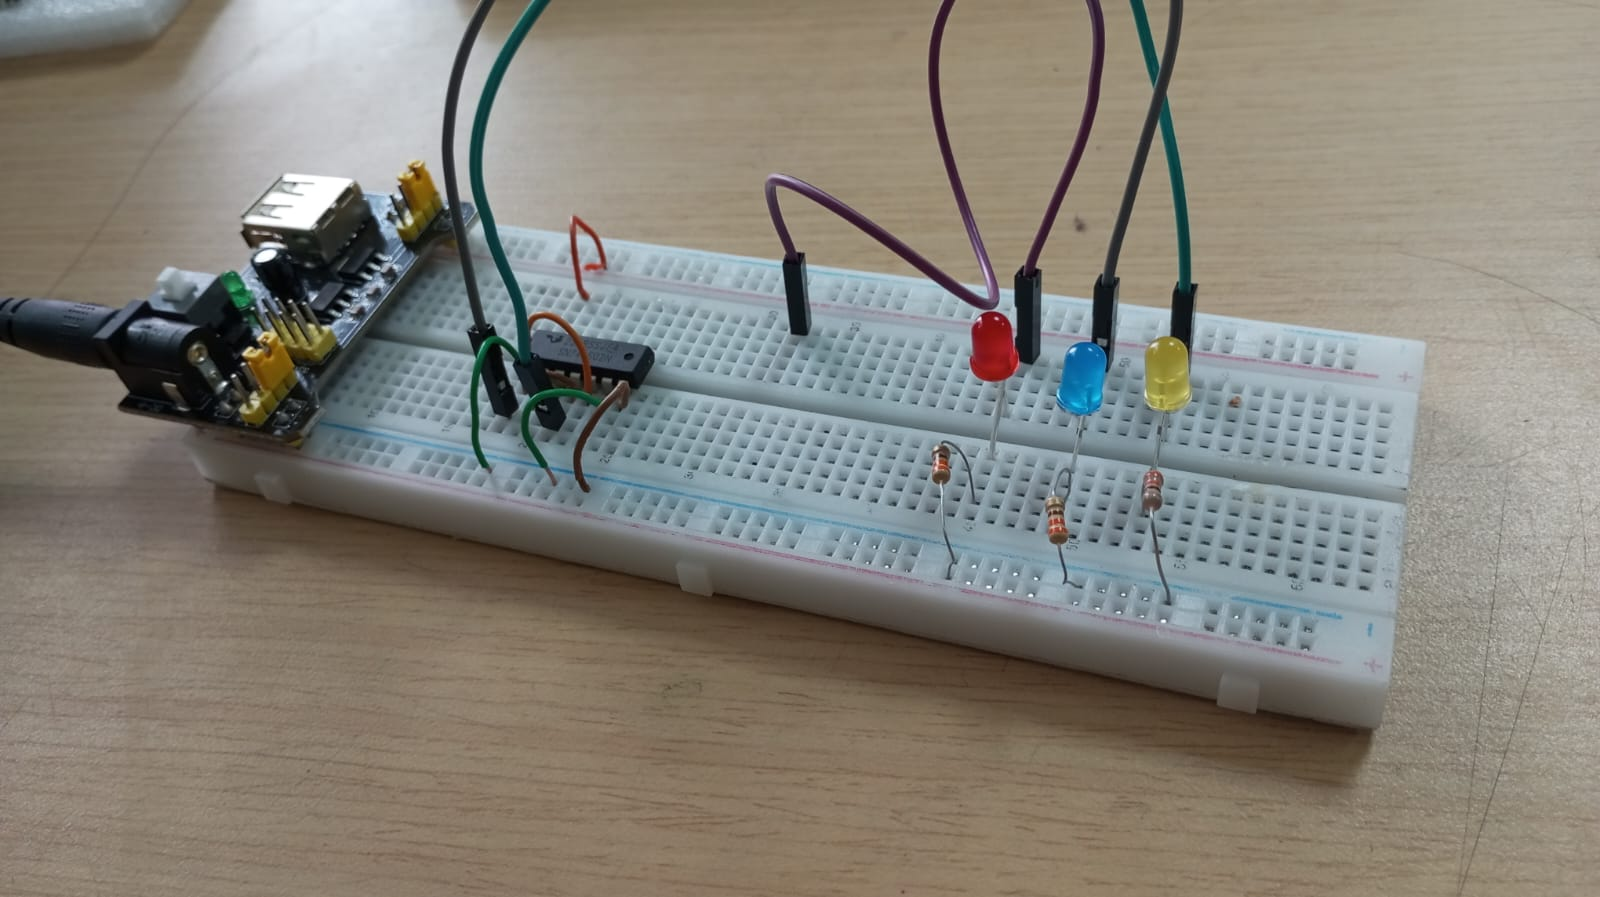
\includegraphics[width=0.8\linewidth]{./Images/basic-latch.jpeg}
	\caption{Montaje de un latch básico.}
	\label{fig:basic-latch}
\end{figure}

En el \Cref{tab:basic-latch} se presentan los resultados obtenidos con el
montaje descrito.

\begin{table}[htbp!]
\centering
\rowcolors{2}{white}{gray!25}
	\begin{tabular}{c|c|c|c}
			\toprule
			B & I & Q & $\bar{\text{Q}}$ \\
			\midrule
			0 & 0 & $\text{Q}_0$ & $\bar{\text{Q}}_0$ \\
			0 & 1 & 0 & 1 \\
			1 & 0 & 1 & 0 \\
			1 & 1 & 0 & 0 \\
			\bottomrule
	\end{tabular}
	\caption{Tabla de resultados del latch construido.}
	\label{tab:basic-latch}
\end{table}

\subsection{Análisis de resultados}
La tabla de resultados es idéntica a los resultados esperados de un flip-flop
SR donde las señales I y B funcionan como R y como S respectivamente.

\subsection{Conclusiones}
Se evidencia que es posible construir un flip-flop SR utilizando únicamente dos
compuertas NOR.

\section{Flip-Flops RS, JK y D}

\section{Flip-Flops D y T}

\section{Construcción de Flip-Flop de Forma Discreta}
\subsection{Montaje y tabla de verdad}
Se construyó un flip-flop JK aparir del uso de compuertas NAND y OR con entradas negadas.
La \Cref{fig:discrete-jk} muestra el diagrama del circuito lógico como también
el detector de flanco derecho para la señal de reloj.
El detector permite que el flip-flop cambie de estado solo cuando la señal de
reloj presente un aumento, esto se puede evidenciar con la \Cref{fig:jk-signal}.

\begin{figure}[h!]
	\centering
	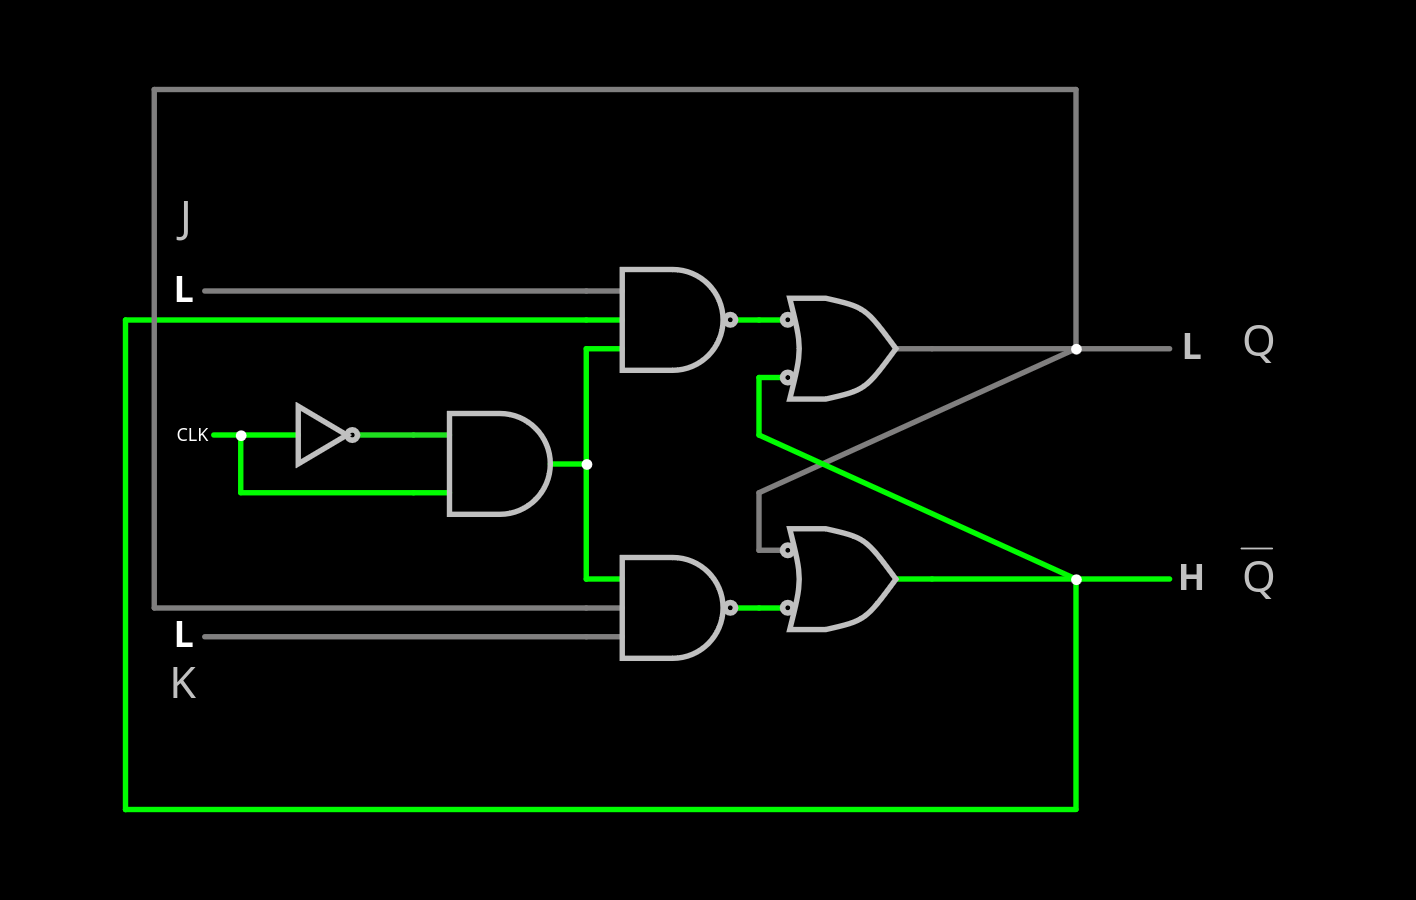
\includegraphics[width=0.8\linewidth]{./Discrete-FF/ff-jk-circuit.png}
	\caption{Diagrama del flip-flop jk construido de forma discreta.}
	\label{fig:discrete-jk}
\end{figure}

\begin{figure}[h!]
	\centering
	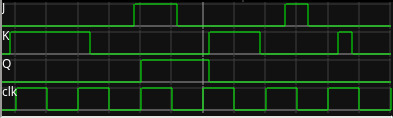
\includegraphics[width=0.8\linewidth]{./Discrete-FF/oscilloscope.jpeg}
	\caption{Señal tomada del osciloscopio.}
	\label{fig:jk-signal}
\end{figure}

A partir del montaje se obtuvieron los resultados que se presentan en el
\Cref{tab:discrete-jk} de forma simplificada.

\begin{table}[h!]
	\centering
	\rowcolors{2}{white}{gray!25}
	\begin{tabular}{c|c|c||c|c}
		\toprule
		CLK & J & K & Q & $\bar{\text{Q}}$ \\
		\midrule
		\RaisingEdge & 0 & 0 & $\text{Q}_{0}$ & $\bar{\text{Q}}_{0}$ \\
		\RaisingEdge & 0 & 1 & 0 & 1 \\
		\RaisingEdge & 1 & 0 & 1 & 0 \\
		\RaisingEdge & 1 & 1 & $\bar{\text{Q}}_{0}$ & $\text{Q}_{0}$ \\
		\bottomrule
	\end{tabular}
	\caption{Tabla de resultados. (Simplificada)}
	\label{tab:discrete-jk}
\end{table}

\subsection{Análisis de resultados}
Los datos obtenidos muestran el mismo comportamiento de un flip-flop JK, tal
como se deseaba, sin embargo, este solo presenta cambios cuando la señal de
reloj aumenta, por esto, el estado (H, H) es semi estable, donde las señales
de salida oscilan hasta terminar en el valor opuesto que tenían en un principio.

Además, se observa que el comportamiento del flip-flop está influenciado
significativamente por el retardo de la compuerta negadora en el detector de
flanco derecho, así como por la frecuencia de la señal. Para hacer evidente este
efecto, se utilizó una señal de \qty{120}{Hz} y un retardo de la compuerta
negadora de aproximadamente \qty{400}{Vs^{-1}}.

\subsection{Conclusiones}
A partir de la combinación de compuertas simples fue posible construir un flip-flop
JK que actualice su estado actual cuando la señal de reloj aumenta, esto haciendo
uso de la no instantáneidad de las señales. El flip-flop construido se comporto
idénticamente a un JK normal sin embargo presenta cambios muy rápidos en el estado
(H, H).

\printbibliography
\nocite{*}

\end{document}
